\mainmatter%
\setcounter{page}{1}

\lectureseries[\course]{\course}

\auth[\lecAuth]{Lecturer: \lecAuth\\ Scribe: \scribe}
\date{December 3, 2009}

\setaddress%

% the following hack starts the lecture numbering at 18
\setcounter{lecture}{17}
\setcounter{chapter}{17}

\lecture{Convexity}

\section{Max-Plus Review}
Last lecture we saw that
\begin{align*}
a\oplus b &\doteq \max\{a,b\} \\
a\otimes b &\doteq a+b \\
\mathbb{R}^- &\doteq \mathbb{R}\cup\{-\infty\}
\end{align*}

\section{Convexity}
Let $\mathcal{C}(\mathbb{R}^n)$ be the space of convex functions mapping $\mathbb{R}^n\to\mathbb{R}^-$.
If $\vp\in\mathcal{C}(\mathbb{R}^n)$ then
$$\vp(\lambda x+(1-\lambda)y) \leq \lambda\vp(x) + (1-\lambda)\vp(y)~\forall x,y\in\mathbb{R}^n,~\forall \lambda\in[0,1]$$

In a previous homework we showed that if $\vp,\psi\in\mathcal{C}(\mathbb{R}^n)$ then
$$[\vp\oplus\psi](x) = \max[\vp(x),\psi(x)], \qquad \vp\oplus\psi\in\mathcal{C}(\mathbb{R}^n)$$

Let $\vp\in\mathcal{C}(\mathbb{R}^n)$ and $c\in\mathbb{R}$.
Is $c\otimes\vp\in\mathcal{C}(\mathbb{R}^n)$?
\begin{align*}
[c\otimes\vp](\lambda x+(1-\lambda)y) &= c\otimes\vp(\lambda x+(1-\lambda)y) \\
&= c + \vp(\lambda x+(1-\lambda)y) \\
&\leq \lambda c + (1-\lambda)c + \lambda\vp(x) + (1-\lambda)\vp(y) \\
&= \lambda[c+\vp(x)] + (1-\lambda)[c+\vp(y)] \\
&= \lambda[c\otimes\vp](x) + (1-\lambda)[c\otimes\vp](y)
\end{align*}
This implies that $\mathcal{C}(\mathbb{R}^n)$ is a max-plus vector space.
However, value functions are generally semi-convex where $\vp$ is semi-convex with constant $\beta\in\mathbb{R}$ if
$$\vp(x) + \frac{\beta}{2}|x|^2$$
is convex.
We will denote $S_\beta(\mathbb{R}^n)$ to be the space of semi-convex functions with constant $\beta$.

\begin{example}
Let $\beta=1$, then
$$-\tfrac{1}{4}{(x-2)}^2\in S_\beta(\mathbb{R})$$
because
$$-\tfrac{1}{4}{(x-2)}^2 + \tfrac{1}{2}x^2 = \tfrac{1}{4}x^2 + x - 1$$
is convex due to the positive coefficient for the $x^2$ term.
See Figure~\ref{fig:18semiconvex}.
$\lozenge$
\end{example}

\begin{figure}[ht!]
\centering
\includegraphics[width=.4\textwidth]{images/18semiconvex}
\caption{A semi-convex function.}
\label{fig:18semiconvex}
\end{figure}

\section{Convex Duality}
Let $a(p)$ be the dual of $\vp(x)$, where $a(p)$ is also known as the Legendre transfer and is given by
\begin{align*}
a(p) &= \min_x\{\vp(x)-p\cdot x\} \\
&= -\max_x\{p\cdot x-\vp(x)\} \\
\vp(x) &= \max_{p\in\mathbb{R}^n}\{a(p)+p\cdot x\} \\
a(p) &= -\int_{\mathbb{R}^n}^\oplus (p\cdot x)\otimes[-\vp(x)]dx \\
\vp(x) &= \int_{\mathbb{R}^n}^\oplus (p\cdot x)\otimes a(p)dp
\end{align*}

\section{Semi-Convex Duality}
Let $\vp\in S_\beta(\mathbb{R}^n)$ and $z=-\frac{\beta}{2}|x-z|^2$, then
\begin{align*}
a(x) &= \min_x\left\lbrace \vp(x) - \tfrac{\beta}{2}|x-z|^2 \right\rbrace \\
\vp(x) &= \max_{z\in\mathbb{R}^n}\left\lbrace a(z) - \tfrac{\beta}{2}|x-z|^2 \right\rbrace
\end{align*}
Let $\psi(x,z)\doteq -\tfrac{\beta}{2}|x-z|^2$, then
\begin{align*}
a(z) &= \min_x\{\vp(x)-\psi(x,z)\} \\
&= -\max\{\psi(x,z)\otimes-\vp(x)\} \\
&= -\int_{\mathbb{R}^n}^\oplus \psi(x,z)\otimes[-\vp(x)]dx \\
\vp(x) &= \int_{\mathbb{R}^n}^\oplus \psi(x,z)\otimes a(z)dz
\end{align*}
This looks like a Laplace transform, we are just using different definitions for addition and multiplication.

Now, instead of looking at all $z$ we will only look at a dense subset such that ${\{z_n\}}_{n=1}^\infty$ is dense in $\mathbb{R}^n$ (dense like the natural numbers).
Then
$$\vp(x) = \max_n\{a(z_n) + \psi(x,z_n)\}$$
where
$$a(z_n) = \int_{\mathbb{R}^n}^\oplus \psi(x,z_n)\otimes [-\vp(x)]dx$$
Let $\hat{a}_n=a(z_n)$ and $\hat{\psi}_n=\psi(x,z_n)$, then
\begin{align}
\label{eq:18vpx}
\vp(x) = \max_n\{\hat{a}_n\otimes\hat{\psi}_n(x)\} = \bigoplus_{n=1}^\infty[\hat{a}_n\otimes\hat{\psi}_n(x)]
\end{align}
with
$$\hat{a}_n = \int_{\mathbb{R}^n}^\oplus \hat{\psi}_n(x)\otimes [-\vp(x)]dx$$
This is like Fourier transforms but in a different space.

${\{\psi_n\}}_{n=1}^\infty$ form a max-plus basis for $S_\beta(\mathbb{R}^n)$.
Since the value functions are all semi-convex we can use $\{\psi_n\}$ to look for the value functions.

\section{Dynamic Programming Application}
We are trying to solve the DPP $V=\mathcal{S}_\delta[V]$, with $\mathcal{S}_\delta$ being max-plus linear.
Suppose that
$$V(x)\simeq \bigoplus_{n=1}^N\hat{a}_n\otimes\hat{\psi}_n(x)$$
and
\begin{align}
\label{eq:18mp}
\bigoplus_{n=1}^N\hat{a}_n\otimes\hat{\psi}_n(x) &\simeq V(x) = \mathcal{S}_\delta[V](x) \nonumber \\
&= \mathcal{S}_\delta\left[\bigoplus_{i=1}^N\hat{a}_i\otimes\hat{\psi}_i(\cdot)\right](x) \nonumber \\
&= \bigoplus_{i=1}^N\hat{a}_i\otimes\mathcal{S}_\delta[\hat{\psi}_i(\cdot)](x)
\end{align}

(\ref{eq:18mp}) has a function of $x$ that can be expanded using the dual because $\mathcal{S}_\delta[\psi_i(\cdot)]$ is a semi-convex function of $x$.
The coefficients for the expansion can be found offline.

By (\ref{eq:18vpx}) we have
$$\mathcal{S}_\delta[\hat{\psi}_i](x) = \bigoplus_{j=1}^N B_{j,i}\otimes\hat{\psi}_j(x)$$
where $B_{j,i}$ are the coefficients and are given by
\begin{align}
\label{eq:18bji}
B_{j,i} = -\max_x\left\lbrace \hat{\psi}_j(x) - \mathcal{S}_\delta[\hat{\psi}_i](x) \right\rbrace
\end{align}
Note that we only need to compute $B_{j,i}$ for $z_j$ close to $z_i$.
By substituting (\ref{eq:18bji}) into (\ref{eq:18mp}) we get
\begin{align*}
\bigoplus_{n=1}^N\hat{a}_n\otimes\hat{\psi}_n(x) &= \bigoplus_{i=1}^N\hat{a}_i\otimes\left[ \bigoplus_{j=1}^N B_{j,i}\otimes\hat{\psi}_j(x)\right] \\
&= \bigoplus_{i=1}^N\left[\bigoplus_{j=1}^N\hat{a}_i\otimes B_{j,i}\otimes \hat{\psi}_j(x)\right] \\
&= \bigoplus_{j=1}^N\left[\bigoplus_{i=1}^N\hat{a}_i\otimes B_{j,i}\otimes \hat{\psi}_j(x)\right] \\
&= \bigoplus_{j=1}^N\left[\bigoplus_{i=1}^N B_{j,i}\otimes\hat{a}_i\right] \otimes \hat{\psi}_j(x)
\end{align*}
Since this is true for all $x$ the result is
$$\hat{a}_n = \bigoplus_{i=1}^N B_{n,i}\otimes\hat{a}_i~\forall n$$

We can use this to build a coefficient vector and matrix where
\begin{align*}
\vec{a} = \left[\begin{array}{c} \hat{a}_1 \\ \hat{a}_2 \\ \vdots \\ \hat{a}_N \end{array}\right], \qquad
B = \left[\begin{array}{c c c c} B_{1,1} & B_{1,2} & \cdots & B_{1,N} \\ B_{2,1} & B_{2,2} & \cdots & B_{2,N} \\ \vdots & \vdots & \vdots & \ddots \\ B_{N,1} & B_{N,2} & \cdots & B_{N,N} \end{array}\right]
\end{align*}
This leads to $\vec{a} = B\otimes\vec{a}$ and now all we need to do is find the max-plus eigenvector $\vec{a}$.

Note that we cannot take the inverse because no additive inverse exists so $B^{-1}$ does not exist.
Instead we will use the max-plus power method.

\subsection{Max-plus Power Method}
Start with $\vec{a}^0$.
Given $\vec{a}^k$ let $\vec{a}^{k+1}=B\otimes\vec{a}^k$.
If $\vec{a}^k\to\vec{a}$ then $\vec{a}^{k+1}\to\bar{\vec{a}}$ where $\bar{\vec{a}}=B\otimes\bar{\vec{a}}$.
This will work if
\begin{itemize}
\item There exists a $j$ such that $B_{j,j}=0$.
\item All other loop sums are negative.
\end{itemize}

\begin{example}
Let
$$B = \left[\begin{array}{c c c} 0 & 1 & 0.5 \\ -3 & -1 & -0.3 \\ -1 & 0.1 & -0.1 \end{array}\right]$$
Let the directed graph have transition costs given by $B_{i,j}$.
Instead of probabilities when using Markov chains the max-plus power method uses costs for going from one node to another.% chktex 35
We can see that $B_{1,1}=0$ and
\begin{align*}
&1\to2\to1 = 1-3 = -2<0 \\
&1\to2\to3\to3\to1 = 1-0.3-0.1-1 < 0
\end{align*}
We need all of those loop sums to be negative and this $B$ was created to do just that.
Now we can use the power method, starting with $\vec{a}^0=0$.
Then
\begin{align*}
\vec{a}^1 &= \left[\begin{array}{c c c} 0 & 1 & 0.5 \\ -3 & -1 & -0.3 \\ -1 & 0.1 & -0.1 \end{array}\right] \left[\begin{array}{c} 0 \\ 0 \\ 0 \end{array}\right] = \left[\begin{array}{c} \max\{0,1,0.5\} \\ \max\{-3,-1,-0.3\} \\ \max\{-1,0.1,-0.1\} \end{array}\right] = \left[\begin{array}{c} 1 \\ -0.3 \\ 0.1 \end{array}\right] \\
\vec{a}^2 &= \left[\begin{array}{c c c} 0 & 1 & 0.5 \\ -3 & -1 & -0.3 \\ -1 & 0.1 & -0.1 \end{array}\right] \left[\begin{array}{c} 1 \\ -0.3 \\ 0.1 \end{array}\right] = \left[\begin{array}{c} 1 \\ -0.2 \\ 0 \end{array}\right]
\end{align*}
This procedure eventually converges in four steps to
$$\vec{a} = \left[\begin{array}{c c c} 1 & -0.3 & 0 \end{array}\right]^T$$
Using this $\vec{a}$ we can reconstruct
$$V (x) = \bigoplus_{i=1}^N\hat{a}_i\otimes~\hat{\psi}_i (x)$$
$\lozenge$
\end{example}% chktex 16
